\newcommand{\proseD}{Let $(\Omega, \mathcal{F}, \mathbb{P})$ be a probability space and $(\mathcal{F}_t)_{t \geq 0}$ a filtration. For a stopping time $\tau$ with $\mathbb{E}[\tau] < \infty$ and increments $X_t$ bounded by $c$, the stopped sum $S_\tau = \sum_{t \le \tau} X_t$ has mean $\mathbb{E}[\tau]\,\mu$, where $\mu = \mathbb{E}[X_1]$, by Wald's identity. This is the only place the boundedness of the increments is used.}
\newcommand{\proseE}{In the regime $k \ll n$ the sketch has $O(k \log n)$ rows, each of which is computed in time $O(\mathrm{nnz}(A))$, so the total cost is $O(\mathrm{nnz}(A) k \log n + n k^2)$. The second term dominates only when $k > \mathrm{nnz}(A)/n \cdot \log n$, which does not happen for the matrices of Section~2.}

\section{Preliminaries}
\proseD

\proseE
For every $x$ in the domain we have
\[
f(x) \le g(x) + \epsilon \quad \text{for all } x \in \mathcal{X},
\]
and so the comparison holds uniformly. The simplest case is
\[
x = y.
\]
\proseD

\begin{lemma}\label{lem:split}
For all $a, b \geq 0$ and $p > 1$,
\begin{equation}\label{eq:split}
\begin{split}
(a+b)^p &\le 2^{p-1}(a^p + b^p) \\
&\le 2^{p}\max(a,b)^p.
\end{split}
\end{equation}
In particular the map $t \mapsto t^p$ is quasi-additive with constant $2^{p-1}$:
\begin{align*}
\|u + v\|_p^p &\le 2^{p-1}\bigl(\|u\|_p^p + \|v\|_p^p\bigr), \\
\|u - v\|_p^p &\ge 2^{1-p}\|u\|_p^p - \|v\|_p^p.
\end{align*}
\end{lemma}

\begin{proof}
By convexity of $t \mapsto t^p$ we have $\left(\frac{a+b}{2}\right)^p \le \frac{a^p + b^p}{2}$, which is the first inequality; the second is immediate.
\end{proof}

\proseE
Two equations in a row, each with its own number:
\begin{equation}\label{eq:first}
\mathcal{R}_n(\mathcal{F}) = \mathbb{E}_\sigma \Bigl[\sup_{f \in \mathcal{F}} \frac{1}{n}\sum_{i=1}^n \sigma_i f(z_i)\Bigr]
\end{equation}
\begin{equation}\label{eq:second}
\sup_{f \in \mathcal{F}} \bigl|R(f) - \widehat{R}(f)\bigr| \le 2\mathcal{R}_n(\mathcal{F}) + \sqrt{\frac{\log(1/\delta)}{2n}}
\end{equation}
\proseD

\begin{figure}[t]
\centering
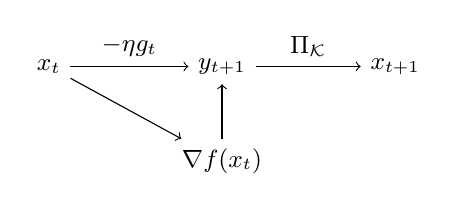
\begin{tikzpicture}[node distance=2.2cm, every node/.style={font=\small}]
\node (a) {$x_t$};
\node[right of=a] (b) {$y_{t+1}$};
\node[right of=b] (c) {$x_{t+1}$};
\node[below of=b, node distance=1.2cm] (d) {$\nabla f(x_t)$};
\draw[->] (a) -- node[above] {$-\eta g_t$} (b);
\draw[->] (b) -- node[above] {$\Pi_{\mathcal{K}}$} (c);
\draw[->] (a) -- (d);
\draw[->] (d) -- (b);
\end{tikzpicture}
\caption{One step of the method: a gradient step to $y_{t+1}$ and a projection back onto $\mathcal{K}$.}
\label{fig:step}
\end{figure}

\section{Analysis}
\proseE
In appendix notation the key estimate is
\begin{equation}
\Bigl\| \sum_{i=1}^{n} \xi_i A_i \Bigr\| \le \sqrt{2 \sigma^2 \log(2d/\delta)} + \frac{2L}{3}\log(2d/\delta) \tag{A.1}
\end{equation}
and the variance proxy is $\sigma^2 = \bigl\|\sum_i \mathbb{E} A_i^2\bigr\|$. Collecting terms, with limits under the operators,
\begin{equation}\label{eq:limits}
\lim_{n \to \infty} \frac{1}{n} \log \Pr\Bigl[\frac{S_n}{n} \ge a\Bigr] = -\sup_{\lambda \ge 0}\bigl(\lambda a - \Lambda(\lambda)\bigr) = -\Lambda^*(a),
\end{equation}
\proseD
\begin{itemize}
\item The first claim follows from
\[
\underbrace{\sum_{k=1}^{m} \binom{m}{k} p^k (1-p)^{m-k}}_{\text{probability of at least one success}} = 1 - (1-p)^m .
\]
\item The second is a direct computation.
\end{itemize}

\begin{table}[t]
\centering
\caption{Running time of the algorithms, with $k$ the target rank.}
\label{tab:time}
\begin{tabular}{lcc}
\toprule
Algorithm & Time & Space \\
\midrule
Exact SVD & $O(n^3)$ & $O(n^2)$ \\
Sketch & $O(\mathrm{nnz}(A) k \log n)$ & $O(nk)$ \\
Ours & $O(\mathrm{nnz}(A) + n k^2)$ & $O(nk)$ \\
\bottomrule
\end{tabular}
\end{table}

\proseE
Old-style arrays still appear in some papers:
\begin{eqnarray}
\Phi(z) & = & \int_{-\infty}^{z} \phi(t)\, dt, \\
\phi(t) & = & \frac{1}{\sqrt{2\pi}} e^{-t^2/2}.
\end{eqnarray}
\proseD
\begin{alignat}{2}
\min_{x}\quad & c^\top x & \qquad & \text{subject to } Ax = b, \label{eq:lp1}\\
& x \ge 0, && x \in \mathbb{Z}^n. \label{eq:lp2}
\end{alignat}
\proseE

\begin{figure}[t]
\centering
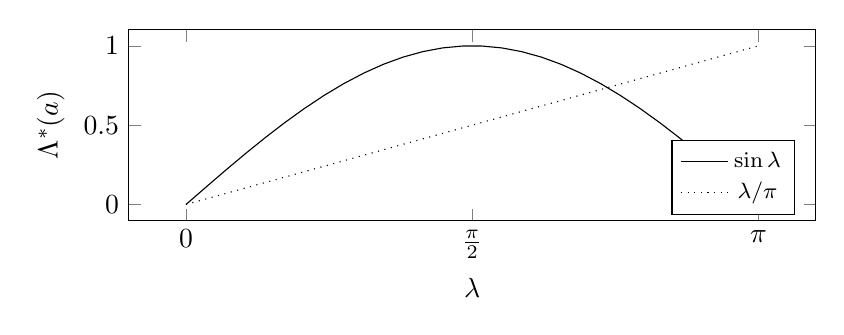
\begin{tikzpicture}
\begin{axis}[width=0.85\linewidth, height=4cm, xlabel={$\lambda$}, ylabel={$\Lambda^*(a)$}, xtick={0,1.5708,3.1416}, xticklabels={$0$,$\frac{\pi}{2}$,$\pi$}, legend pos=south east, legend style={font=\footnotesize}]
\addplot[domain=0:3.1416, samples=30] {sin(deg(x))};
\addlegendentry{$\sin \lambda$}
\addplot[domain=0:3.1416, samples=30, dotted] {x/3.1416};
\addlegendentry{$\lambda / \pi$}
\end{axis}
\end{tikzpicture}
\caption{The rate function against $\lambda$.}
\end{figure}

\proseD
A display with tall delimiters:
\begin{equation}\label{eq:tall}
\left( \sum_{i=1}^n \left| \frac{x_i - \bar{x}}{s} \right|^p \right)^{1/p} \le n^{1/p} \max_{1 \le i \le n} \frac{|x_i - \bar{x}|}{s}.
\end{equation}
\proseE
